\dev{Emile Martinez}{Daphné Kany}

\textit{Cette leçon présente une (ou éventuellement 2 suivant le temps qu'on met à la faire) approximation gloutonne de Indep(2). On suppose ici la définition formelle de Indep déjà faites dans le plan de cours}

\paragraph{Instance} n tâches de durée $\omega_1, \dots \omega_n$
\paragraph{Pb} Trouver un ordonnancement sur $P_1, P_2$ qui minimise la date de fin $\tau$

\begin{algorithm}[H]
$\tau_1, \,\tau_2 \leftarrow 0$ \quad\# date de fin de $P_1,\,P_2$ \\
\Pour{i allant de $1$ à $n$}
{
	\eSi{$\tau_1 \leq \tau_2$}{
		$alloc[i] \leftarrow 1$\\
		$\sigma[i] \leftarrow \tau_1$\\
		$\tau_1 = \tau_1 + \omega_i$\\
	}{
		\#idem avec $\tau_1 \leftrightarrow \tau_2$\\
	}
}
\Retour{$\max (\tau_1, tau_2)$}
\caption{Glouton-1($w_1, \dots, w_n$)}
\end{algorithm}

\begin{proposition}
	Glouton-1 n'est pas optimal.
\end{proposition}

\begin{proof}
	Soit $I$ une l'instance $\omega_1 = \omega_2 = 1$ et $\omega_3 = 2$. On obtient alors\\
	\begin{minipage}{0.4\linewidth}
		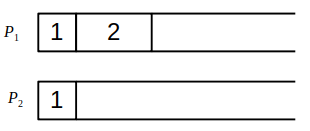
\includegraphics[scale = 0.5]{Developpements/Glouton indep 2/instance1.png} 
	\end{minipage}
	\begin{minipage}{0.4\linewidth}
		$\tau = \tau_1 = 3 \newline \tau^* = 2$
	\end{minipage}
\end{proof}

\begin{theorem}
	Glouton-1 est une $\frac{3}{2}$-approx de Indep(2)
\end{theorem}

\begin{proof}
	$\bullet$ D'abord, Glouton-1 est bien polynomial\\
	
	$\bullet$ Soit I une instance. On note $\tau$ la réponse de Glouton-1, $\tau^*$ l'optimal.
	
	Il faut alors montrer que $\dfrac{\tau}{\tau^*} \leq \dfrac{3}{2}$
	
	\paragraph{Intuition}\begin{minipage}{0.4\linewidth}
	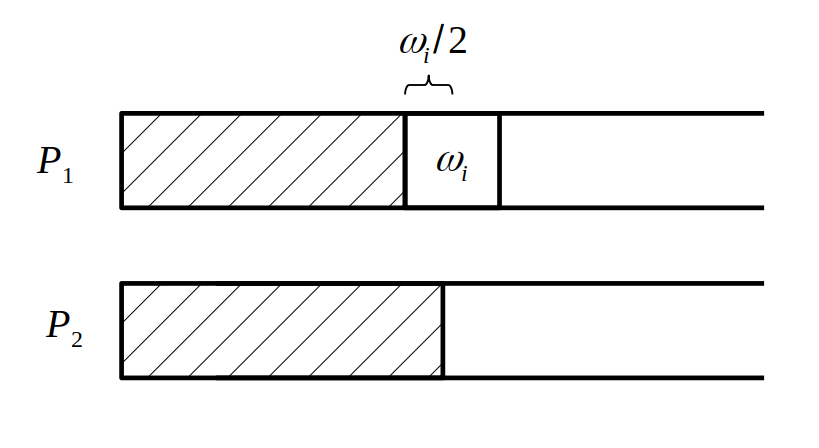
\includegraphics[scale=0.2]{Developpements/Glouton indep 2/instance2.png}\end{minipage}
	\begin{minipage}{0.4\linewidth}
		$\tau = \tau_1$ \\ $\tau^* \geq \tau - \omega_i + \frac{\omega_i}{2}$\\$ \tau \leq \frac{3\tau^*}{2}$
	\end{minipage}
	
	\begin{com}
		Ici pour expliquer, on commence par dire que on suppose que le processeur le plus occupé c'est le 1, puis on regarde la dernière tâche qu'on a mis dessus. Alors, quand on l'a mise, $P_2$ était plus avancé. Donc, ce moment là est plus grand que $\tau^*$ sans $\omega_i$. Or quand on va rajouter $\omega_i$, au mieux on pourra ne rajouter que $\frac{\omega_i}{2}$ à chacun des processeurs en réorganisant. Donc $\tau^*$ avec $\omega_i$ c'est au moins $\tau^*$ sans $\omega_i$, plus $\frac{\omega_i}{2}$, donc $\underset{\leq \tau^* \text{ sans } \omega_i}{\underbrace{\tau - \omega_i}} + \frac{\omega_i}{2}$
	\end{com}
	
	\paragraph{Preuve de l'intuition} On note $S = \sum\limits_{i = 1}^n \omega_i$
	$$\tau^* \geq \dfrac{S}{2} \qquad \circled{1}$$
	
	$$\tau_1 + \tau_2 = S \qquad \circled 2$$
	
	On considère $\tau = \tau_1$, et $\omega_i$ est la dernière tâche de $P_1$.\\
	Au moment de l'insertion de $\omega_1$ : $\underset{= \tau - \omega_i}{\underbrace{\tau_1^{(i)}}} \leq \tau^{(i)} \leq \tau^{(i)} $ \quad \circled 3\\
	
	$$\circled 3 \quad \tau_1 \leq \tau_2 - \omega_i \underset{\circled 2}{\leq} S - \tau_1 + \omega_i$$
	
	$$ 2\tau_1 \leq \underset{\leq 2\tau^* \enspace \circled 1}{\underbrace{S}} + \underset{\leq \tau^*}{\underbrace{\omega_i}} \leq 3\tau^* $$
	
\end{proof}

\begin{algorithm}[H]
	$w_1, \dots, w_n \leftarrow$ Tri($\omega_1, \dots, \omega_n$)\\
	\Retour{Glouton-1($w_1, \dots, w_n$)} 
\caption{Glouton-2($\omega_1, \dots, \omega_n$)}
\end{algorithm}

\begin{theorem}
	Glouton-2 est une $\frac{7}{6}$-approx
\end{theorem}

\begin{proof}
	On reprend la preuve de Glouton-1, mais en essayant d'améliorer $\tau^* \geq \omega_i$
	\begin{itemize}[label=$\star$]
		\item Soit $i \leq 4$, Glouton-2 est optimal\\
		$\to$ Faire tous les cas.\begin{com}
			Si il reste du temps, dire que parce que soit il faut mettre une tâche toute seule, et on le fait, soit il faut mettre la plus grande avec la plus petite, et on le fait.
		\end{com}
		\item Sinon $i \geq 5$. Alors, on a $\tau^* \geq 3 \omega_i$ (Car il y a un ruban avec 3 éléments valant au moins $\omega_i$). D'où $2\tau_1 \leq 2\tau^* + \dfrac{\tau^*}{3}$ i.e. $\tau \leq \dfrac{7}{6}\tau^*$
	\end{itemize}
\end{proof}

\paragraph{Exemple où la borne est atteinte}
Sur l'instance $\omega_1 = \omega_2 = 3$ et $\omega_3 = \omega_4 = \omega_5 = 2$, on obtient\\
	\raisebox{-0.5\height}{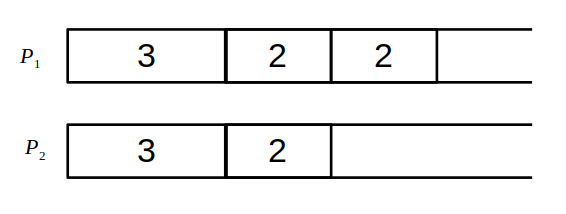
\includegraphics[scale = 0.3]{Developpements/Glouton indep 2/instance4.png}} au lieu de 
	\raisebox{-0.5\height}{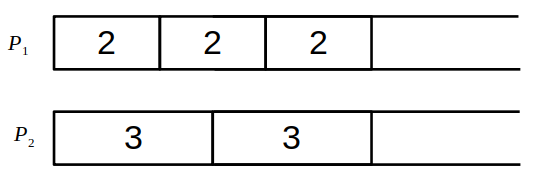
\includegraphics[scale = 0.3]{Developpements/Glouton indep 2/instance3.png}}


\begin{rem}
	Avec Glouton-2 on perd la propriété d'être en ligne. \\
	Avec Glouton-2, l'approx est mauvaise surtout pour les cas où on a peu de tâches. On pourrait alors combiner une approche exhaustive pour les premières tâches, et une approche gloutonne pour les petites.
\end{rem}

\begin{com}
	Si on a du temps, on peut aussi parler de ce qui se passe quand on a plus de processeur. On peut dire sur le dessin, que $\omega_i$ se répartit sur plus de processeurs, et donc $\tau^* \geq \tau_1 - \omega_i + \frac{\omega_i}{p}$. Ca nous fait au final une $2-\frac{1}{p}$ approx pour Glouton-1 et une $\frac{4p-1}{3p}$ pour Glouton-2
\end{com}